\documentclass{beamer}
\usepackage{graphicx}
\usepackage{xcolor}
\usepackage{tikz}
\usepackage{amsmath}
\usepackage{pgfplots}
\pgfplotsset{compat=1.18}

\definecolor{purpleblue}{RGB}{80, 80, 180}
\definecolor{novelPurple}{RGB}{98, 54, 255}
\definecolor{softPurple}{RGB}{180, 170, 255}
\definecolor{softGray}{RGB}{235, 235, 245}
\definecolor{lightText}{RGB}{90, 90, 110}

\usetheme{Madrid}
\usecolortheme{dolphin}
\graphicspath{{static/course_materials/}{static/hard/}{./}}

\setbeamerfont{title}{size=\Large,series=\bfseries}
\setbeamerfont{frametitle}{size=\LARGE,series=\bfseries}
\setbeamercolor{frametitle}{fg=white, bg=novelPurple}
\setbeamercolor{title}{fg=white, bg=purpleblue}

\title[Test VI]{\textbf{Test VI}}
\author{\textbf{Jack Zeng}}
\institute{\textcolor{white}{\textbf{Novel Prep}}}
\date{\today}

\begin{document}

\begin{frame}
    \titlepage
    \vfill
    \begin{flushright}
        \textcolor{purpleblue}{\Huge \textbf{Novel Prep}}
    \end{flushright}
\end{frame}

\begin{frame}
    \begin{tikzpicture}[remember picture, overlay]
        \shade[top color=softPurple, bottom color=softGray]
            (current page.north west) rectangle (current page.south east);
        \node[align=center] at (current page.center) {
            {\Huge\bfseries\textcolor{purpleblue}{Novel Prep}} \\[0.5cm]
            {\Large\itshape\textcolor{lightText}{Phase 3 · Mock Exam Training}}
        };
    \end{tikzpicture}
\end{frame}

\begin{frame}{Overview}
    \tableofcontents
\end{frame}

\begin{frame}
\section{Test VI}
    \begin{tikzpicture}[remember picture, overlay]
        \shade[top color=softPurple, bottom color=softGray]
            (current page.north west) rectangle (current page.south east);
        \node[align=center] at (current page.center) {
            {\LARGE\bfseries\textcolor{purpleblue}{Test VI}} \\[0.5cm]
            {\Large\itshape\textcolor{lightText}{20 error-prone Module 2-style practice questions}}
        };
    \end{tikzpicture}
\end{frame}

% --- Question 1 ---
\begin{frame}{Question 1}
\small
Hector used a tool called an auger to remove corn from a storage bin at a constant rate. The bin contained 24,000 bushels of corn when Hector began to use the auger. After 5 hours of using the auger, 19,350 bushels of corn remained in the bin. If the auger continues to remove corn at this rate, what is the total number of hours Hector will have been using the auger when 12,840 bushels of corn remain in the bin?
\vspace{0.35cm}
\begin{enumerate}
    \item[A.] 3
    \item[B.] 7
    \item[C.] 8
    \item[D.] 12
\end{enumerate}
\end{frame}
\begin{frame}{Answer 1}
\small
\textbf{Correct Answer:} D
\end{frame}

% --- Question 2 ---
\begin{frame}{Question 2}
\small
\begin{center}
\textbf{Townsend Realty Group Investments}

\renewcommand{\arraystretch}{1.3}
\begin{tabular}{|l|c|c|}
\hline
\textbf{Property address} & \textbf{Purchase price (dollars)} & \textbf{Monthly rental price (dollars)} \\
\hline
Clearwater Lane & 128{,}000 & 950 \\
Driftwood Drive & 176{,}000 & 1{,}310 \\
Edgemont Street & 70{,}000 & 515 \\
Glenview Street & 140{,}000 & 1{,}040 \\
Hamilton Circle & 450{,}000 & 3{,}365 \\
\hline
\end{tabular}
\end{center}

The Townsend Realty Group invested in the five different properties listed in the table above. The table shows the amount, in dollars, the company paid for each property and the corresponding monthly rental price, in dollars, the company charges for the property at each of the five locations.

Townsend Realty purchased the Glenview Street property and received a 40\% discount off the original price along with an additional 20\% off the discounted price for purchasing the property in cash. Which of the following best approximates the original price, in dollars, of the Glenview Street property?
\vspace{0.35cm}
\begin{enumerate}
    \item[A.] \$350{,}000
    \item[B.] \$291{,}700
    \item[C.] \$233{,}300
    \item[D.] \$175{,}000
\end{enumerate}
\end{frame}
\begin{frame}{Answer 2}
\small
\textbf{Correct Answer:} B
\end{frame}

% --- Question 3 ---
\begin{frame}{Question 3}
\small
Each side of a 30-sided polygon has one of three lengths. The number of sides with length 8 \textbf{centimeters (cm)} is 5 times the number of sides \( n \) with length 3 cm. There are 6 sides with length 4 cm. Which equation must be true for the value of \( n \)?
\vspace{0.35cm}
\begin{enumerate}
    \item[A.] $5n + 6 = 30$
    \item[B.] $6n + 6 = 30$
    \item[C.] $8n + 3n + 4n = 30$
    \item[D.] $8(5n) + 3n + 4(6) = 30$
\end{enumerate}
\end{frame}
\begin{frame}{Answer 3}
\small
\textbf{Correct Answer:} B
\end{frame}

% --- Question 4 ---
\begin{frame}{Question 4}
\small
A window repair specialist charges \textbf{\$220} for the first two hours of repair plus an hourly fee for each additional hour. The total cost for 5 hours of repair is \textbf{\$400}. Which function \( f \) gives the total cost, in dollars, for \( x \) hours of repair, where \( x \geq 2 \)?
\vspace{0.35cm}
\begin{enumerate}
    \item[A.] $f(x) = 60x + 100$
    \item[B.] $f(x) = 60x + 220$
    \item[C.] $f(x) = 80x$
    \item[D.] $f(x) = 80x + 220$
\end{enumerate}
\end{frame}
\begin{frame}{Answer 4}
\small
\textbf{Correct Answer:} A
\end{frame}

% --- Question 5 ---
\begin{frame}{Question 5}
\small
One gallon of paint will cover 220 square feet of a surface. A room has a total wall area of \( w \) square feet. Which equation represents the total amount of paint \( P \), in gallons, needed to paint the walls of the room twice?
\vspace{0.35cm}
\begin{enumerate}
    \item[A.] $P = \frac{w}{110}$
    \item[B.] $P = 440w$
    \item[C.] $P = \frac{w}{220}$
    \item[D.] $P = 220w$
\end{enumerate}
\end{frame}
\begin{frame}{Answer 5}
\small
\textbf{Correct Answer:} A
\end{frame}

% --- Question 6 ---
\begin{frame}{Question 6}
\small
A laundry service is buying detergent and fabric softener from its supplier. The supplier will deliver no more than 300 pounds in a shipment. Each container of detergent weighs 7.35 pounds, and each container of fabric softener weighs 6.2 pounds. The service wants to buy at least twice as many containers of detergent as containers of fabric softener. Let \( d \) represent the number of containers of detergent, and let \( s \) represent the number of containers of fabric softener, where \( d \) and \( s \) are nonnegative integers. Which of the following systems of inequalities best represents this situation?
\vspace{0.35cm}
\begin{enumerate}
    \item[A.] $7.35d + 6.2s \leq 300$, \\ \hspace*{1.5em} $d \geq 2s$
    \item[B.] $7.35d + 6.2s \leq 300$, \\ \hspace*{1.5em} $2d \geq s$
    \item[C.] $14.7d + 6.2s \leq 300$, \\ \hspace*{1.5em} $d \geq 2s$
    \item[D.] $14.7d + 6.2s \leq 300$, \\ \hspace*{1.5em} $2d \geq s$
\end{enumerate}
\end{frame}
\begin{frame}{Answer 6}
\small
\textbf{Correct Answer:} A
\end{frame}

% --- Question 7 ---
\begin{frame}{Question 7}
\small
The triangle inequality theorem states that the sum of any two sides of a triangle must be greater than the length of the third side. If a triangle has side lengths of $6$ and $12$, which inequality represents the possible lengths, $x$, of the third side of the triangle?
\vspace{0.35cm}
\begin{enumerate}
    \item[A.] $x < 18$
    \item[B.] $x > 18$
    \item[C.] $6 < x < 18$
    \item[D.] $x < 6 \text{ or } x > 18$
\end{enumerate}
\end{frame}
\begin{frame}{Answer 7}
\small
\textbf{Correct Answer:} C
\end{frame}

% --- Question 8 ---
\begin{frame}{Question 8}
\small
What is the smallest solution to the equation  
\[
\sqrt{(x - 2)^2} = \sqrt{3x + 34}
\]
\end{frame}
\begin{frame}{Answer 8}
\small
\textbf{Final Answer:} $\boxed{-3}$
\end{frame}

% --- Question 9 ---
\begin{frame}{Question 9}
\small
The population $P$ of a certain city $y$ years after the last census is modeled by the equation  
$P = P_0(1 + r)^y$, where $r$ is a constant and $P_0$ is the population when $y = 0$.  
If the population decreases each year by a fixed percent, which of the following must be true?
\vspace{0.35cm}
\begin{enumerate}
    \item[A.] $r < -1$
    \item[B.] $-1 < r < 0$
    \item[C.] $0 < r < 1$
    \item[D.] $r > 1$
\end{enumerate}
\end{frame}
\begin{frame}{Answer 9}
\small
\textbf{Correct Answer:} B
\end{frame}

% --- Question 10 ---
\begin{frame}{Question 10}
\small
\begin{center}
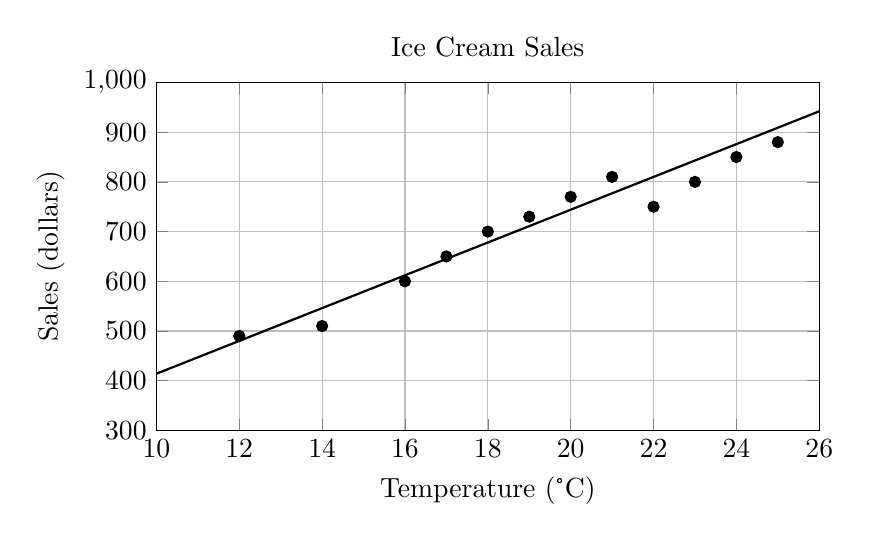
\begin{tikzpicture}
\begin{axis}[
    xlabel={Temperature (°C)},
    ylabel={Sales (dollars)},
    ytick={300,400,...,1000},
    xmin=10, xmax=26,
    ymin=300, ymax=1000,
    grid=major,
    width=10cm, height=6cm,
    title={Ice Cream Sales}
]
\addplot[
    only marks,
    mark=*,
]
coordinates {
    (12, 490)
    (14, 510)
    (16, 600)
    (17, 650)
    (18, 700)
    (19, 730)
    (20, 770)
    (21, 810)
    (22, 750)
    (23, 800)
    (24, 850)
    (25, 880)
};
\addplot[domain=10:26, thick] {33*x + 84};
\end{axis}
\end{tikzpicture}

\end{center}

The scatterplot above shows a company’s ice cream sales $d$, in dollars, and the high temperature $t$, in degrees Celsius (°C), on 12 different days.  
A line of best fit for the data is also shown.  
Which of the following could be an equation of the line of best fit?
\vspace{0.35cm}
\begin{enumerate}
    \item[A.] $d = 0.03t + 402$
    \item[B.] $d = 10t + 402$
    \item[C.] $d = 33t + 300$
    \item[D.] $d = 33t + 84$
\end{enumerate}
\end{frame}
\begin{frame}{Answer 10}
\small
\textbf{Correct Answer:} D
\end{frame}

% --- Question 11 ---
\begin{frame}{Question 11}
\small
For $x > 0$, the function $f$ is defined as follows:  
\begin{center}

$f(x)$ equals $201\%$ of $x$.
\end{center}

Which of the following could describe this function?
\vspace{0.35cm}
\begin{enumerate}
    \item[A.] Decreasing exponential
    \item[B.] Decreasing linear
    \item[C.] Increasing exponential
    \item[D.] Increasing linear
\end{enumerate}
\end{frame}
\begin{frame}{Answer 11}
\small
\textbf{Correct Answer:} D
\end{frame}

% --- Question 12 ---
\begin{frame}{Question 12}
\small
\begin{center}
    

\textbf{Poll Results}

\begin{tabular}{|l|c|}
\hline
Candidate & Votes \\
\hline
Angel Cruz & 483 \\
Terry Smith & 320 \\
\hline
\end{tabular}
\end{center}

The table shows the results of a poll. A total of 803 voters selected at random were asked which candidate they would vote for in the upcoming election.  
According to the poll, if 6,424 people vote in the election, by how many votes would Angel Cruz be expected to win?
\vspace{0.35cm}
\begin{enumerate}
    \item[A.] 163
    \item[B.] 1,304
    \item[C.] 3,864
    \item[D.] 5,621
\end{enumerate}
\end{frame}
\begin{frame}{Answer 12}
\small
\textbf{Correct Answer:} B
\end{frame}

% --- Question 13 ---
\begin{frame}{Question 13}
\small
The given equation is one equation in a system of two linear equations.  
If the system of equations has at least one solution, which of the following equations could be the other equation in the system?

\[
7x + 5y = 2
\]

\begin{itemize}
    \item[I.] \(10.5x + 7.5y = 3\)
    \item[II.] \(10.5x - 7.5y = 3\)
\end{itemize}
\vspace{0.35cm}
\begin{enumerate}
    \item[A.] I only
    \item[B.] II only
    \item[C.] I and II
    \item[D.] Neither I nor II
\end{enumerate}
\end{frame}
\begin{frame}{Answer 13}
\small
\textbf{Correct Answer:} C
\end{frame}

% --- Question 14 ---
\begin{frame}{Question 14}
\small
In a set of four consecutive odd integers, where the integers are ordered from least to greatest, the first integer is represented by $x$. The product of 28 and the third odd integer in the set is at most the value of 50 less than the sum of the first and fourth odd integers in the set. What is the greatest possible value of $x$?
\vspace{0.35cm}
\begin{enumerate}
    \item[A.] $-5$
    \item[B.] $-6$
    \item[C.] $-7$
    \item[D.] $-8$
\end{enumerate}
\end{frame}
\begin{frame}{Answer 14}
\small
\textbf{Correct Answer:} C
\end{frame}

% --- Question 15 ---
\begin{frame}{Question 15}
\small
The functions \(f\) and \(g\) are defined by the equations shown, where \(a\) and \(b\) are integer constants, \(a < b\), and \(b < 0\). If \(y = f(x)\) and \(y = g(x)\) are graphed in the \(xy\)-plane, which of the following equations displays, as a constant or coefficient, the \(y\)-coordinate of the \(y\)-intercept of the graph of the corresponding function?

\begin{itemize}
    \item[I.] \(f(x) = a(2.1)^{x + b}\)
    \item[II.] \(g(x) = a(2.1)^x + b\)
\end{itemize}
\vspace{0.35cm}
\begin{enumerate}
    \item[A.] I only
    \item[B.] II only
    \item[C.] I and II
    \item[D.] Neither I nor II
\end{enumerate}
\end{frame}
\begin{frame}{Answer 15}
\small
\textbf{Correct Answer:} D
\end{frame}

% --- Question 16 ---
\begin{frame}{Question 16}
\small
The positive number \(a\) is 2,106\% of the sum of the positive numbers \(b\) and \(c\),  
and \(b\) is 81\% of \(c\).  

What percent of \(b\) is \(a\)?
\vspace{0.35cm}
\begin{enumerate}
    \item[A.] 4,706\%
    \item[B.] 47.06\%
    \item[C.] 470600\%
    \item[D.] 47060\%
\end{enumerate}
\end{frame}
\begin{frame}{Answer 16}
\small
\textbf{Correct Answer:} A
\end{frame}

% --- Question 17 ---
\begin{frame}{Question 17}
\small
In one hour, the distance, \(d(s)\), in kilometers that a ferry can travel up and down a river  
flowing with a constant speed \(s\), in meters per second, is:  
\[
d(s) = 10.7 - 1.2s^2
\]  
where \(s\) and \(d(s)\) are positive.  

Which of the following equivalent expressions for \(d(s)\) contains the speed  
of the river in meters per second, as a constant or coefficient, for which  
the ferry can travel a distance of 8 kilometers in one hour?
\vspace{0.35cm}
\begin{enumerate}
    \item[A.] \(8 - 1.2(s - 1.5)(s + 1.5)\)
    \item[B.] \(8 + 1.2(2.25 - s^2)\)
    \item[C.] \(8(1 - 0.15s^2) + 2.7\)
    \item[D.] \(11.9 - 1.2(s - 1)^2 - 2.4s\)
\end{enumerate}
\end{frame}
\begin{frame}{Answer 17}
\small
\textbf{Correct Answer:} A
\end{frame}

% --- Question 18 ---
\begin{frame}{Question 18}
\small
Given the quadratic equation:  
\[
7rx^2 - 28sx + 7r
\]  
In the equation:  
\begin{itemize}
  \item \(r\) is a positive constant  
  \item \(s\) is a negative constant  
  \item The equation has two solutions  
\end{itemize}

If \( \frac{r}{s} > k \), what is the minimum value of \(k\)?
\end{frame}
\begin{frame}{Answer 18}
\small
\textbf{Final Answer:} $\boxed{-2}$
\end{frame}

% --- Question 19 ---
\begin{frame}{Question 19}
\small
The speed of a vehicle is increasing at a rate of $7.3$ meters per second squared. What is this rate, in \textbf{miles per minute squared}, rounded to the nearest tenth? (Use $1$ mile $= 1{,}609$ meters.)
\vspace{0.35cm}
\begin{enumerate}
    \item[A.] $0.3$
    \item[B.] $16.3$
    \item[C.] $195.8$
    \item[D.] $220.4$
\end{enumerate}
\end{frame}
\begin{frame}{Answer 19}
\small
\textbf{Correct Answer:} B
\end{frame}

% --- Question 20 ---
\begin{frame}{Question 20}
\small
A sociologist chose 300 students at random from each of two schools and asked each student how many siblings he or she has. The results are shown in the table below:

\begin{center}
\begin{tabular}{|c|c|c|}
\hline
\textbf{Number of siblings} & \textbf{Lincoln School} & \textbf{Washington School} \\
\hline
0 & 120 & 140 \\
1 & 80 & 110 \\
2 & 60 & 30 \\
3 & 30 & 10 \\
4 & 10 & 10 \\
\hline
\end{tabular}
\end{center}

There are a total of 2,400 students at Lincoln School and 3,300 students at Washington School. Based on the survey data, which of the following most accurately compares the expected total number of students with 4 siblings at the two schools?
\vspace{0.35cm}
\begin{enumerate}
    \item[A.] The total number of students with 4 siblings is expected to be equal at the two schools.
    \item[B.] The total number of students with 4 siblings at Lincoln School is expected to be 30 more than at Washington School.
    \item[C.] The total number of students with 4 siblings at Washington School is expected to be 30 more than at Lincoln School.
    \item[D.] The total number of students with 4 siblings at Washington School is expected to be 900 more than at Lincoln School.
\end{enumerate}
\end{frame}
\begin{frame}{Answer 20}
\small
\textbf{Correct Answer:} C
\end{frame}

\begin{frame}{}
    \begin{tikzpicture}[remember picture, overlay]
        \shade[top color=novelPurple!40, bottom color=white]
            (current page.north west) rectangle (current page.south east);
        \fill[white, opacity=0.15] (current page.center) circle (5cm);
        \foreach \x in {1,2,3,4,5} {
            \fill[novelPurple, opacity=0.12] (rand*10-5, rand*7-3.5) circle (0.1+\x*0.05);
        }
    \end{tikzpicture}
    \centering
    \vspace{5em}
    {\Huge \textbf{\textcolor{novelPurple}{Thank You!}}} \\[1em]
    {\large \textcolor{gray}{We appreciate your time and focus.}} \\[3em]
    {\LARGE \textbf{\textcolor{novelPurple}{\textsf{Novel Prep}}}}
    \vfill
\end{frame}

\end{document}
